\begin{wrapfigure} [11]{r}{0.47\textwidth}
  \centering
  \vspace{-0.4cm}
  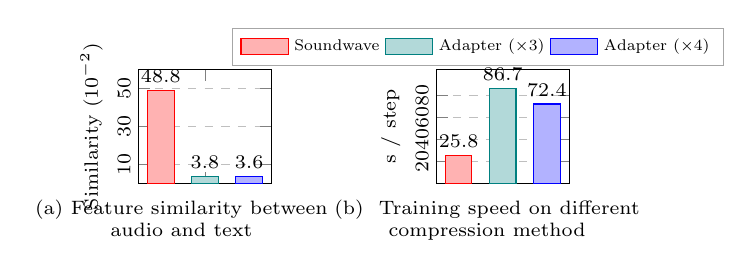
\begin{tikzpicture}
    \scriptsize
    \begin{axis}[
      ymajorgrids,
      grid style=dashed,
      ybar=3pt,
      enlarge x limits=0.5,
      xtick align=inside,
      height=.25\textwidth,
      width=.27\textwidth, 
      bar width=1.2em,
      xlabel={(a) Feature similarity between\\ audio and text},
      xlabel style={xshift=-0.3cm},
      ylabel={Similarity ($10^{-2}$)},
      xtick=data,
      symbolic x coords={A-T}, 
      nodes near coords,  
      nodes near coords align={vertical},
      ymin=0,
      ymax=60,
      ytick={10,30,50},
      xticklabels={
        {} 
      },
      x tick label style={align=center, font=\tiny}, 
      xlabel style={yshift=0.3em,align=center},
      yticklabel style={,rotate=90},
    ]
    every node near coord/.append style={  
        font=\tiny,  
        /pgf/number format/.cd,  
        fixed,  
        fixed zerofill,  
        precision=2  
    }  
    

      \addplot[bar shift=-2em, fill=red!30, draw=red, area legend] coordinates {
        (A-T, 48.8) 
      };
      \addplot[fill=teal!30, draw=teal, area legend] coordinates {
        (A-T, 3.8) 
      };
      \addplot[bar shift=2em, fill=blue!30, draw=blue, area legend] coordinates {
        (A-T, 3.6) 
      };
      \legend{};
    \end{axis}
    
    \scriptsize{
    \begin{axis}[
      at={(13.5em,0)},
      ymajorgrids,
      grid style=dashed,
      legend style={draw=gray!70, at={(-1.535,1.03)}, anchor=south west},
      legend columns=3,
      legend cell align={left},
      ybar,
      enlarge x limits=0.5,
      xtick align=inside,
      height=.25\textwidth,
      width=.27\textwidth,
      bar width=1.2em,
      xlabel={(b) \ Training speed on different\\compression method},
      ylabel={s / step},
      xlabel style={xshift=-0.2cm},
      symbolic x coords={{1}, {2}},
      xtick=data,
      nodes near coords,
      nodes near coords align={vertical},
      ymin=0,
      ymax=104,
      ytick={20, 40, 60, 80},
      xticklabels={},
      legend entries={Soundwave, Adapter ($\times3$), Adapter ($\times4$)},
      xlabel style={yshift=0.3em,align=center},
      yticklabel style={rotate=90},
      ]
      \addplot[bar shift=-2em, fill=red!30, draw=red, area legend] coordinates {
        ({1}, 25.8) 
      };
      \addlegendentry{\scalebox{.8}{Soundwave}}

      \addplot[fill=teal!30, draw=teal,area legend] coordinates {({1},86.7)};
      \addlegendentry{\scalebox{.8}{Adapter ($\times3$)}} 
      
      \addplot[bar shift=2em, fill=blue!30, draw=blue,area legend] coordinates {({1},72.4)}; 
      \addlegendentry{\scalebox{.8}{Adapter ($\times4$)}}  
    \end{axis}
    }
\end{tikzpicture}
\vspace{-0.5cm}
\caption{Comparison of alignment effects and training speeds of different methods.}
\label{denosieperformance}

\end{wrapfigure} 